%% other_works_licenses.tex 
%%
%% Presentation of the course ``Legal Issues'' of the Official Master on Libre Software (URJC)
%% http://master.libresoft.es
%%


%%%%%%%%%%%%%%%%%%%%%%%%%%%%%%%%%%%%%%%%%%%%%%%%%%%%%%%%%%%%%%%%%%%%%%%
\section{Lesson IV: Free licenses for other intellectual works}
%%%%%%%%%%%%%%%%%%%%%%%%%%%%%%%%%%%%%%%%%%%%%%%%%%%%%%%%%%%%%%%%%%%%%%%


%%%%%%%%%%%%%%%%%%%%%%%%%%%%%%%%%%%%%%%%%%%%%%%%%%%%%%%%%%%%%%%%%%%%%%%

\begin{frame}
\frametitle{Free Licenses for other intellectual works}

\begin{itemize}
\item FLOSS licenses have inspired licenses for other intellectual
  works: audio, video\ldots 

\item Stallman distinguished between \alert{functional works} (documentation, encyclopedias, manuals, etc.), and \alert{non-functional works} (literature, music, movies, etc.) to justify the use of restrictive clauses for works other than software.\\\pause

\end{itemize}

\end{frame}

%%%%%%%%%%%%%%%%%%%%%%%%%%%%%%%%%%%%%%%%%%%%%%%%%%%%%%%%%%%%%%%%%%%%%%%
\begin{frame}
\frametitle{Functional Works vs. non-functional Works}
\begin{itemize}
\item Is it true that non-functional works require less freedoms? \\\pause

\item Legitimation of non-commercial clauses? (and other restrictive clauses).
\end{itemize}                                                 

\end{frame}


%%%%%%%%%%%%%%%%%%%%%%%%%%%%%%%%%%%%%%%%%%%%%%%%%%%%%%%%%%%%%%%%%%%%%%%
\begin{frame}
\frametitle{What is a free culture?}
\begin{itemize}
\item ``Free culture'' as in ``free speech'', ``free markets'', ``free  trade'', ``free enterprise''. ``free will'' and ``free elections''.
\item A free culture supports and protects creators and innovators: no es nada nuevo, es la forma tradicional en que se ha construido nuestra cultura.
\item A free culture is not a culture without property, just as a free market is not a
market in which everything is free. 
\item  The opposite of a free culture is a ``permission culture'' --a culture in which creators get to create only with the permission of the powerful, or of creators from the past. (L. Lessig)

\end{itemize}

\end{frame}

%%%%%%%%%%%%%%%%%%%%%%%%%%%%%%%%%%%%%%%%%%%%%%%%%%%%%%%%%%%%%%%%%%%%%%%

\begin{frame}
\frametitle{Controversy about definition of free cultural works}

\begin{itemize}
\item \alert{Freedom Defined}: There isn't free culture without the right to make derivative works or commercial uses.
\item \alert{Lax use}: accepting limitations to transform works or to trade with them.
\end{itemize}                                                 

\end{frame}




%%%%%%%%%%%%%%%%%%%%%%%%%%%%%%%%%%%%%%%%%%%%%%%%%%%%%%%%%%%%%%%%%%%%%%%

\begin{frame}
\frametitle{``Freedom Defined'': free cultural works}

\begin{itemize}
\item It's not a new license, but an initiative to provide a definition of \alert{free} outside of the software world to end the current ambiguity of the term in the Free Culture movement.
\item CC fails to establish a ``base level of freedom'' (Mako Hill)
\item A Debian developer proposal (Mako Hill): reached consensus over a draft with the community, the FSF and CC. 
\item It's an adaptation of the four essential freedoms of Free Software.
\item It's not about the author's right to decide the terms in which he wants to share his work, it is about getting knowledge of which licenses (and works) do or do not fit the definition of \alert{free}.
\end{itemize}                                                 

\end{frame}


%%%%%%%%%%%%%%%%%%%%%%%%%%%%%%%%%%%%%%%%%%%%%%%%%%%%%%%%%%%%%%%%%%%%%%%

\begin{frame}
\frametitle{``Freedom Defined'': Definition of Freedom}

By \alert{freedom} we mean:

\begin{itemize}
\item the \alert{freedom to use} the work and enjoy the benefits of using it
\item the \alert{freedom to study} the work and to apply knowledge acquired from it
\item the \alert{freedom to make and redistribute copies}, in whole or in part, of the information or expression
\item the \alert{freedom to make changes and improvements}, and to distribute derivative works 
\end{itemize}                                                 

\end{frame}

%%%%%%%%%%%%%%%%%%%%%%%%%%%%%%%%%%%%%%%%%%%%%%%%%%%%%%%%%%%%%%%%%%%%%%%

\begin{frame}
\frametitle{Defining Free Cultural Works}

These are the additional conditions in order for a work to be considered free:

\begin{itemize}
\item \alert{Availability of source data} (score of a musical composition, the models used in a 3D scene, the data of a scientific publication, the source code of a computer application, or any other such information)
\item \alert{Use of a free format} (no patents)
\item \alert{No technical restrictions}
\item \alert{No other restrictions or limitations:} The work itself must not be covered by legal restrictions (patents, contracts, etc.) or limitations which would impede the freedoms enumerated above.
\end{itemize}                                                 

\end{frame}


%%%%%%%%%%%%%%%%%%%%%%%%%%%%%%%%%%%%%%%%%%%%%%%%%%%%%%%%%%%%%%%%%%%%%%%

\begin{frame}
\frametitle{Identifying Free Cultural Works}

Whenever the user of a work cannot legally or practically exercise his basic freedoms, the work cannot be considered and should not be called ``free''. So: 

\begin{itemize}
\item \alert{Non-commercial} restrictions are \alert{non-free} licenses.
\item \alert{No derivative} restrictions are \alert{non-free} licenses. 
\item \alert{Non-Commercial Share-alike} Is Not Copyleft: Copyleft is a reversal of copyright. It restores and protects the rights that copyright removes. \alert{The} rights, not \textit{some} rights.
\item ``Open Content'' and ``Open Access'' are \alert{not} a clear definition of freedom. 
\end{itemize}                                                 

% \vspace{1cm}
\begin{center}
% {\LARGE
% \textbf{\url{http://freedomdefined.org/}}
% }

\includegraphics[width=2.5cm]{figs/seal.png}

\end{center}


\end{frame}


%%%%%%%%%%%%%%%%%%%%%%%%%%%%%%%%%%%%%%%%%%%%%%%%%%%%%%%%%%%%%%%%%%%%%%%



\begin{frame}
\frametitle{The GNU FDL}

GNU has the ``Free Documentation License'' (GFDL). In this license:
\begin{itemize}
\item There are distinction between ``transparent'' copies of the
  document (similar to ``source'') and ``opaque'' copies (similar to
  ``binary'').
\item There are some additional restrictions: acknowledgments,
  dedications, and the history of the document can be modified but
  only by adding new lines.
\item The document could include ``invariant'' and ``cover'' sections, not
  modifiable. However, only ``non-technical'' texts can be considered
  invariant.
\item GFDL does not comply with Debian guidelines (DRM clause, GPL incompatible and 
invariant parts), unless the invariant section clauses are not used. 

\end{itemize}


\end{frame}

%%%%%%%%%%%%%%%%%%%%%%%%%%%%%%%%%%%%%%%%%%%%%%%%%%%%%%%%%%%%%%%%%%%%%%%

\begin{frame}
\frametitle{Wikipedia Case}

\begin{itemize}
\item Until June 2009, WP contents were covered by the GFDL.
\item Wikipedia was relicensed to CC-by-sa 3.0, another copyleft license.
\item Causes? 

\pause

\small
	\begin{itemize}
		\item The GFDL is not suitable for online reference works (designed for printed works). 
		\item GFDL compliance is almost impossible: to reproduce an excerpt from Wikipedia would need to attach (not binding) to complete the GFDL and contributions throughout history.
		\item No-compatible with the CC-by-sa, copyleft license more widespread.
	\end{itemize}

\end{itemize}

\pause
\begin{center}
\alert{If every author is holder of his/her edition, how could Wikipedia be relicensed?}
\end{center}

\end{frame}



%%%%%%%%%%%%%%%%%%%%%%%%%%%%%%%%%%%%%%%%%%%%%%%%%%%%%%%%%%%%%%%%%%%%%%%

\begin{frame}
\frametitle {How could Wikipedia be relicensed?}

\pause

\begin{itemize}
\item A community referendum in April 2009.
\item GFDL 1.2 ``\alert{or} any later version'' clause
\item At request of the Wikimedia Foundation, FSF released a new GFDL version (1.3), designed
specifically to allow relicense Wikipedia content as CC-by-sa.
\item Conflict with art. 14.1 LPI? (``corresponden al autor los siguientes derechos irrenunciables e \alert{inalienables}: 1. Decidir si su obra ha de ser divulgada y en qué forma'').
\end{itemize}

\end{frame}


%%%%%%%%%%%%%%%%%%%%%%%%%%%%%%%%%%%%%%%%%%%%%%%%%%%%%%%%%%%%%%%%%%%%%%%

\begin{frame}
\begin{center}
\huge{Creative Commons Licenses}
\end{center}

\end{frame}

%%%%%%%%%%%%%%%%%%%%%%%%%%%%%%%%%%%%%%%%%%%%%%%%%%%%%%%%%%%%%%%%%%%%%%%

\begin{frame}
\frametitle{Creative Commons objectives}

Creative Commons, a non-profit organisation for...

\begin{itemize}
\item Creating a set of licenses, for any type of content.
\item Indexing CC licensed works, so you can locate free contents fast...
\item International adaptation of licenses (for example, there are
  Spanish official CC licenses)
\end{itemize}
\vspace{1cm}
\begin{center}
{\LARGE
\textbf{\url{http://www.creativecommons.org/}}
}
\end{center}

\end{frame}

%%---------------------------------------------------------------

\begin{frame}
\frametitle{Creative Common Licenses objectives}

With Creative Common licenses you can...

\begin{itemize}
\item Donate your work to the Public Domain or...
\item Maintain some rights:
\begin{itemize}
\item Attribution
\item Non-commercial
\item No derivative
\item Share Alike
\end{itemize}
\item You can {\bf combine} these rights (with some logical exceptions). So, you maintain
\begin{center}
{\LARGE{\bf some rights reserved}}.
\end{center}
\end{itemize}

\end{frame}

%%---------------------------------------------------------------

\begin{frame}
\frametitle{Creative Commons: Simplicity}

Why CC is so popular:

\begin{itemize}
\item Simple web tool
\item We only have to answer basic questions like: ``Allow commercial uses? Allow modifications?''
\end{itemize}

\end{frame}


%%---------------------------------------------------------------

\begin{frame}
\frametitle{Copyright: All rights reserved}

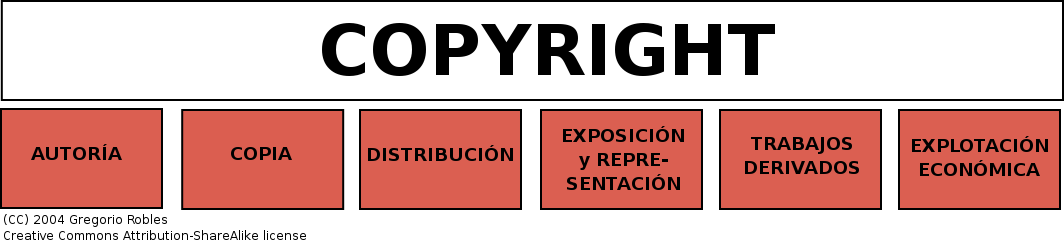
\includegraphics[width=11cm]{figs/Copyright.png}

\end{frame}

%%---------------------------------------------------------------

\begin{frame}
\frametitle{Public Domain: No rights reserved}

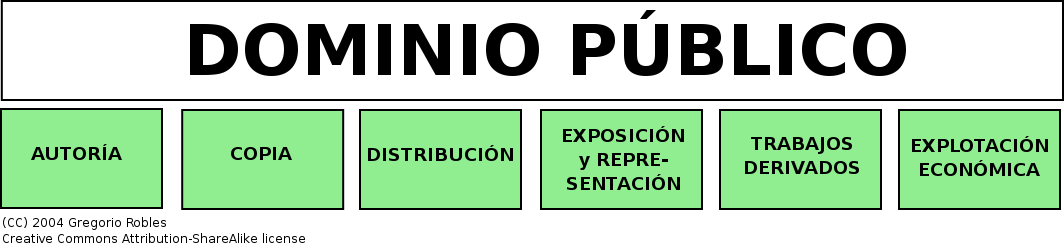
\includegraphics[width=11cm]{figs/DominioPublico.png}

\end{frame}

%%---------------------------------------------------------------

\begin{frame}
\frametitle{Creative Commons: Some rights reserved}

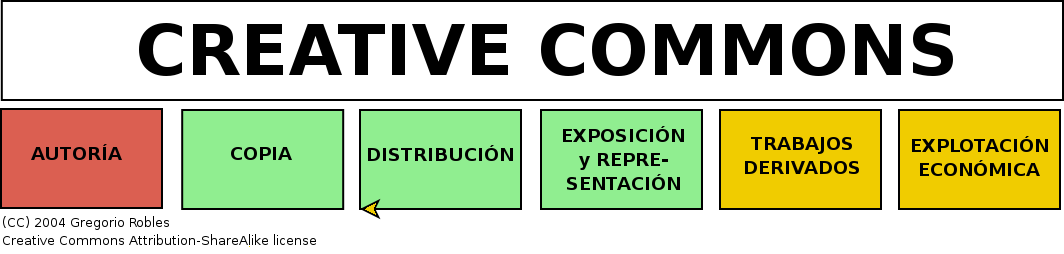
\includegraphics[width=11cm]{figs/CreativeCommons.png}

\end{frame}


%%%%%%%%%%%%%%%%%%%%%%%%%%%%%%%%%%%%%%%%%%%%%%%%%%%%%%%%%%%%%%%%%%%%%%%
\begin{frame}
\frametitle{Types of Creative Commons licenses (1/2)}

Mixing and matching these conditions produces six possible combinations:

\begin{block}{CC Licenses}
\begin{enumerate}
\item Attribution (by)
\item Attribution + Non commercial (by-nc)
\item Attribution + No Derivate Works (by-nd)
\item Attribution + share alike (by-sa)
\item Attribution + Non commercial + No Derivate Works (by-nc-nd)
\item Attribution + Non commercial + share alike (by-nc-sa)
\end{enumerate}                                                 
\end{block}
\end{frame}


%%%%%%%%%%%%%%%%%%%%%%%%%%%%%%%%%%%%%%%%%%%%%%%%%%%%%%%%%%%%%%%%%%%%%%%
\begin{frame}
\frametitle{Types of Creative Commons licenses (2/2)}

``Special'' CC licenses:
\begin{itemize}
\item Public Domain Dedication (and CC0)
\item \alert{Founder's Copyright:} the work is released into PD after 14 or 28 years.
\item \alert{Sampling Plus:} parts of the work can be copied and modified for any purpose. The entire work can be copied for non-commercial purposes.
\item \alert{Noncommercial Sampling Plus:} the whole work or parts of the work can be copied and modified for noncommercial purposes. 
\end{itemize}                                                 

Retired licenses: Developing Nations, Sampling.

\end{frame}

%%%%%%%%%%%%%%%%%%%%%%%%%%%%%%%%%%%%%%%%%%%%%%%%%%%%%%%%%%%%%%%%%%%%%%%
\begin{frame}
\frametitle{Creative Commons and software licenses}

\begin{itemize}
\item CC Licenses weren't designed for use with software: don't make mention of source or object code.
\item CC recommends to use available licenses from the free/open source software world.
\item CC has ``wrapped'' some free software/open source licenses (BSD, GPL and LGPL) with a human-readable ``Commons Deed'' and machine-readable metadata (``three-layer packaging'').
\item It is important to note that CC has not altered these software licenses in any way.
\item GPL and LGPL includes a Portuguese translation (job made for Brazilian government).
\end{itemize}                                                 

\end{frame}


%%%%%%%%%%%%%%%%%%%%%%%%%%%%%%%%%%%%%%%%%%%%%%%%%%%%%%%%%%%%%%%%%%%%%%%
\begin{frame}
\frametitle{Projects with Creative Commons licenses}

\begin{itemize}
\item \alert{Wikipedia} (cc-by-sa, since June 2009)
\item \alert{Wikia} (cc-by-sa, since June 2009). A free web hosting service for wikis
\item \alert{Citizendium} (cc-by-sa). Wiki-based Encyclopedia.
\item \alert{knol} (mostly, cc-by-sa or cc-by-nc-sa). A Google project that aims to include user-written articles on a range of topics
\item \alert{Arduino} (cc-by-sa). A single-board microcontroller and a software suite for programming it. 
\item \alert{NINJAM} (cc-by-sa). A mechanism for exchanging audio data across the internet.
\end{itemize}                                                 

\end{frame}

%%---------------------------------------------------------------


%%%%%%%%%%%%%%%%%%%%%%%%%%%%%%%%%%%%%%%%%%%%%%%%%%%%%%%%%%%%%%%%%%%%%%%
\begin{frame}
\frametitle{Use of Creative Commons licenses}

All CC licenses contain a \alert{three-layer user interface} (for humans, lawyers and machines):
\begin{itemize}
\item \alert{Commons Deed:} It is a summary, human-readable, of the license with the relevant icons.
\item \alert{Legal Code:} The complete legal code in which the chosen license is based.
\item \alert{Digital Code.} The digital code, a machine-readable version that helps search engines and other applications identify the work by its terms of use.
\end{itemize}                                                 

\end{frame}

%%---------------------------------------------------------------

\begin{frame}
\frametitle{The Attribution license}

With this license, you reserve only moral rights:

\begin{itemize}
\item Attribution of your work.
\end{itemize}

There are not restrictions in commercial use or derivative works.

This license is the nearest to a FLOSS permissive license. 

\end{frame}


%%---------------------------------------------------------------

\begin{frame}
\frametitle{The Attribution-ShareAlike license}

With this license, you reserve two rights:

\begin{itemize}
\item Attribution of your work.
\item Any derived work must be licensed under same license.
\end{itemize}

This license is the nearest to a copyleft license. 

\end{frame}

%%---------------------------------------------------------------

\begin{frame}
\frametitle{CC Zero license}


\begin{itemize}
\item Created in 2009.
\item CC0 is the ``no rights reserved'' option (like a PD dedication).
\item Anyone can then use the work in any way and for any purpose
\item Public Domain legally robust way: universal applicability, intended for use world-wide by anyone.
\item If the waiver isn't effective for any reason, then CC0 acts as a license from the affirmer granting the public an unconditional, irrevocable, non exclusive, royalty free license to use the work for any purpose. 
\end{itemize}


\end{frame}

%%---------------------------------------------------------------

\begin{frame}
\frametitle{CC Zero (CC0) -- No Copyright}

\begin{block}{CC0 Public Domain Dedication}
``The person who associated a work with this deed has dedicated the work to the public domain by waiving all of his or her rights to the work worldwide under copyright law, including all related and neighboring rights, to the extent allowed by law.''
\end{block}

\medskip

\small
CC0 rights granted: ``\alert{You can copy, modify, distribute and perform the work, even for commercial purposes, all without asking permission.}''

\end{frame}

%%---------------------------------------------------------------

\begin{frame}
\frametitle{CC Zero (CC0) -- No Copyright}

\begin{center}
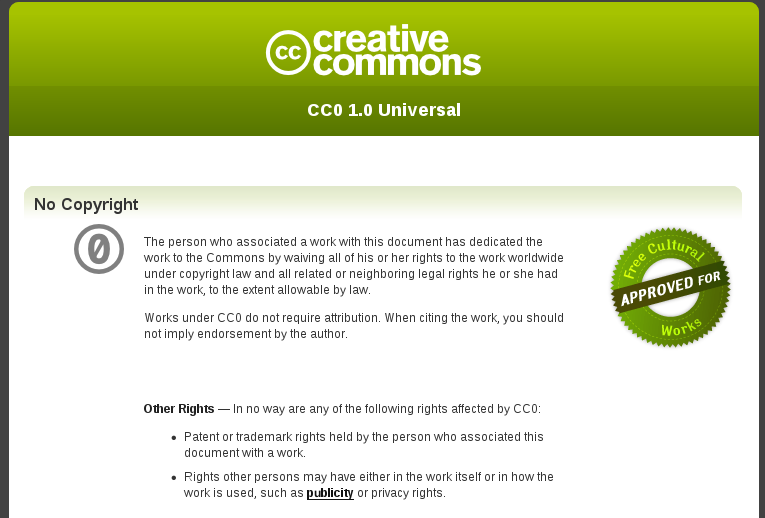
\includegraphics[width=8cm]{figs/cc0.png}
\end{center}


\end{frame}

%%%%%%%%%%%%%%%%%%%%%%%%%%%%%%%%%%%%%%%%%%%%%%%%%%%%%%%%%%%%%%%%%%%%%%%
\begin{frame}
\frametitle{CC NonCommercial Share-alike (CC-nc-sa)}

Is it a free license?
\pause

\begin{itemize}
\item CC-nc-sa is \alert{NOT} a free license.
\end{itemize}                                                 

\pause

Is it a copyleft license?
\pause

\begin{itemize}
\item NonCommercial Share-alike is \alert{NOT} a copyleft license: copyleft rebuilds and protects the rights that restrictive copyright removes.
\item \alert Rights, no \textit{some} rights.
\end{itemize}                                                 

\end{frame}



%%%%%%%%%%%%%%%%%%%%%%%%%%%%%%%%%%%%%%%%%%%%%%%%%%%%%%%%%%%%%%%%%%%%%%%
\begin{frame}
\frametitle{¿What does it mean non-commercial?}

\begin{block}{Noncommercial clause}
\small

You may not exercise any of the rights granted to You [...] in any manner that is primarily intended for or directed toward commercial advantage or private monetary compensation. 



\end{block}

\end{frame}


%%%%%%%%%%%%%%%%%%%%%%%%%%%%%%%%%%%%%%%%%%%%%%%%%%%%%%%%%%%%%%%%%%%%%%%

\begin{frame}
\frametitle{The ``non-commercial'' clause (1/3)}

\begin{itemize}
\item It is frequently used, particularly in blogs and social sites, and it is now being adopted by some institutions.
\item They are believed to protect the work against abusive use and opportunists (reselling or commercial exploitation by corporations, etc.).
\item It is sometimes supported by alleging that protects investment (though some studies have challenged this view, since it restricts distribution).
\end{itemize}                                                 

\end{frame}

%%%%%%%%%%%%%%%%%%%%%%%%%%%%%%%%%%%%%%%%%%%%%%%%%%%%%%%%%%%%%%%%%%%%%%%

\begin{frame}
\frametitle{The ``non-commercial'' clause (2/3)}

It raises evil side effects: 
\begin{itemize}
\item This clause does not distinguish between indirect commercial uses, self-funded projects, etc.
\item It brings uncertainty about what is a commercial activity: when in doubt you might decide not to use it to avoid demands or consulting lawyers... 
\item Incompatibility with libre projects (i.e. Wikipedia).
\item Causing confusion about  the ``free'' concept: it promotes another kind of opportunism, by using viral marketing to create the impression that a work is free but not truly releasing it as a libre product.
\end{itemize}                                                 

\end{frame}

%%%%%%%%%%%%%%%%%%%%%%%%%%%%%%%%%%%%%%%%%%%%%%%%%%%%%%%%%%%%%%%%%%%%%%%

\begin{frame}
\frametitle{The ``non-commercial'' clause (3/3)}

\begin{itemize}
\item The author's right to decide the terms in which he shares his work is not at stake here.
\item What it is rejected is the confusion and the subterfuge of presenting a work as a free product when it is not true.
\item Use any license you like, but also use concepts with accuracy: do not label as \textit{free/libre} or \textit{copyleft} what it is not. Confusion damages free culture and benefit opportunists.
\end{itemize}
\end{frame}

%%%%%%%%%%%%%%%%%%%%%%%%%%%%%%%%%%%%%%%%%%%%%%%%%%%%%%%%%%%%%%%%%%%%%%%

\begin{frame}
\frametitle{Exercise: Choose a license}

\begin{itemize}
\item Choose a CC License for your blog
\end{itemize}
\end{frame}



%%%%%%%%%%%%%%%%%%%%%%%%%%%%%%%%%%%%%%%%%%%%%%%%%%%%%%%%%%%%%%%%%%%%%%%

\begin{frame}
\begin{center}
\huge{Debian Guidelines and Creative Commons Licenses}
\end{center}

\end{frame}


%%---------------------------------------------------------------

\begin{frame}
\frametitle{Debian-legal enters the arena}

After the popularization of CC, Debian-legal warned of
Attribution provisions. The causes were:

\begin{itemize}
\item A work under Attribution can be in fact, NoDerivs 
\item Downstream users remove an author's credit upon request from the author.
\item Inaccurate or excessive authorship credits.
\item Problems with Anti-DRM provisions (which could restrict private redistribution to some extent).
\item Trademark restrictions.
\item Attribution[-ShareAlike] 2.x is NOT compatible with DFSG. 
\item Efforts to fix these problems in the new version 3.0 licenses.

\end{itemize}


\end{frame}



%%---------------------------------------------------------------

\begin{frame}
\frametitle{CC Attribution Problems (I)}

\begin{itemize}
\item Licensor/Original Author can request removal of him/her references in derived works.
\item However the author name must be included in derivative works ``if supplied'' (Attribution)
\end{itemize}

It's unclear if creator of derivative works can comply with a requirement of removing references and requirement of give attribution. Then, a request to remove references can make impossible to comply with Attribution; so it may not be possible to make derivative/collective works under this license (DFSG 3 \& 1 incompatible). {\bf The work is not free?}

\end{frame}

%%---------------------------------------------------------------

\begin{frame}
\frametitle{CC Attribution Problems (II): Authorship credits}

\begin{itemize}
\item Requirements for crediting Licensor for his/her work: it's ambiguous
\item So, we need the most pessimistic interpretation:
\begin{itemize}
\item Required attribution for the licensor everywhere that authorship credit is given.
\end{itemize}
% \item Excessive/Inaccurate authorship credits: DFSG 1 \& 3 incompatible.
\end{itemize}
Example 1: {\it If a work is a collection of essays by different authors, with authorship credit given in the chapter titles, the Licensor's name would have to be listed for each chapter title, even if they did not contribute to it.}\\
Example 2: {\it If Alice writes her autobiography, and includes lyrics from Bob's song in one chapter, she must give him credit for the entire work: ``The Autobiography of Alice, by Alice and Bob'', or even ``The Autobiography of Alice and Bob.''}
\end{frame}

%%---------------------------------------------------------------

\begin{frame}
\frametitle{CC Attribution Problems (III)}

\begin{itemize}
\item Anti-DRM Clause: Distribution with measures to control access is not compatible with DFSG 1.
\end{itemize}

Example 1: Private distribution of work might be forbidden.\\
Example 2: Distribution in a server with control access (i.e. firewall) might be forbidden.
\end{frame}

%%---------------------------------------------------------------

\begin{frame}
\frametitle{CC Attribution Problems (IV)}

\begin{itemize}
\item Web page says: Using CC trademark or logos is strictly prohibited when it's used for other than indicating the work is licensed under CC.
\item Although CC Trademark not appears to be part of the CC licenses, this is only warned in ``source code'' of CC web page.
\item Interpretation: This can prevent redistribution, modification ...
\end{itemize}

\end{frame}

%%---------------------------------------------------------------

\begin{frame}
\frametitle{CC NoDerivs clause problems}

\LARGE{Obviously, NoDerivs licenses are not compatible with Four Freedoms (nor DFSG)}

\end{frame}

%%---------------------------------------------------------------

\begin{frame}
\frametitle{CC NonCommercial clause problems}

\LARGE{Obviously, NonCommercial licenses are not compatible with Four Freedoms (nor DFSG)}

\end{frame}

%%---------------------------------------------------------------


\begin{frame}
\frametitle{Debian recommendations to authors}

\begin{itemize}
\item All software licensed under CC 2.x is NOT compatible with DFSG. 
\item CC 3.x has fixed several of these problems.
\item Software licensed under NonCommercial/NoDerivs can't be named ``Free Software''.
\item Authors who wish to use Attribution must use other licenses as BSD.
\item Authors who wish to use Attribution-ShareAlike must use other licenses as GFDL.
\end{itemize}

\end{frame}


%%---------------------------------------------------------------
%%%%%%%%%%%%%%%%%%%%%%%%%%%%%%%%%%%%%%%%%%%%%%%%%%%%%%%%%%%%%%%%%%%%%%%
% \section{References}
%%%%%%%%%%%%%%%%%%%%%%%%%%%%%%%%%%%%%%%%%%%%%%%%%%%%%%%%%%%%%%%%%%%%%%%

% \begin{frame}
% \frametitle{References}

% \begin{itemize}
% \item \textsc{Van Lindberg}, \textit{Intellectual Property and Open Source}, O'Reilly, July 2008.
% \item \textsc{Malcolm Bain} et al. \textit{Aspectos legales y de explotación del software libre}, UOC, February 2007. \\
% \url{http://ocw.uoc.edu/informatica-tecnologia-y-multimedia/aspectos-legales-y-de-explotacion-del-software-libre/materiales/}
% \item \textsc{Lawrence Rose}, \textit{Open Source Licensing}, Prentice Hall, July 2004 
% \end{itemize}

% \end{frame}


%%%%%%%%%%%%%%%%%%%%%%%%%%%%%%%%%%%%%%%%%%%%%%%%%%%%%%%%%%%%%%%%%%%%%%%


%%---------------------------------------------------------------


%\begin{frame}
%\frametitle{Exercise: Analyze a software public license}

%Search on the web the EUPL License (versions 1.0 and 1.1). Read it in the language of your choice.

%\begin{itemize}
%\item What kind of license is? (Non-free/permissive/recíprocal...)
%\item How does it solve incompatibility with copyleft licenses?
%\item Analyse carefully section 13 of both versions (1.0 and 1.1). What has it been changed? What do you think it was due this change?
%\item Is it applicable outside the EU? What is the geographic scope of the license?
%\item Does it have anti-patent defense? If yes, how is it implemented? (Quoting the passage). How does it work?
%\item Has it Affero clause? Where?
%\end{itemize}

%\end{frame}

